\section{Field strength calculation}
The strength $\mathbf{g}$ of the gravitational field at mesh-point $\mathbf{x}_\mathbf{p}$ can be approximated using a central difference.
Our implementation supports two types of finite differences, defined below as two variants of an particular operator.
\begin{enumerate}
    \item The $j$-th component ($j = x, y, z$) of the two-point finite difference operator $\mathbf{D}$ is given by
          \begin{equation}\label{eq:two-point-central-diff-def-1}
              D_j(\phi)(\mathbf{x}_\mathbf{p}) = \frac{\phi(\mathbf{x}_{p} + H\mathbf{e}_j) - \phi(\mathbf{x}_\mathbf{p} - H\mathbf{e}_j)}{2H},
          \end{equation}
          where $\mathbf{e}_j$ is the $j$-th standard basis vector.
          This scheme is second-order accurate.
    \item The four-point finite difference operator $\mathbf{D}$ is defined in terms of its components $j$ as
          \begin{equation*}
              D_j(\phi)(\mathbf{x}_\mathbf{p}) = \alpha\frac{\phi(\mathbf{x}_{p} + H\mathbf{e}_j) - \phi(\mathbf{x}_\mathbf{p} - H\mathbf{e}_j)}{2H} + (1-\alpha)\frac{\phi(\mathbf{x}_\mathbf{p} + 2H\mathbf{e}_j) - \phi(\mathbf{x}_\mathbf{p} - 2H\mathbf{e}_j)}{4H}.
          \end{equation*}
          The scheme is fourth-order accurate for $\alpha = 4/3$.
\end{enumerate}

The difference between the accuracy of both methods is illustrated in \autoref{fig:finite-diff-accuracy}.
The figure also provides insight into how the error depends on the value of parameter $\alpha$.
\begin{figure}[htp]
    \centering
    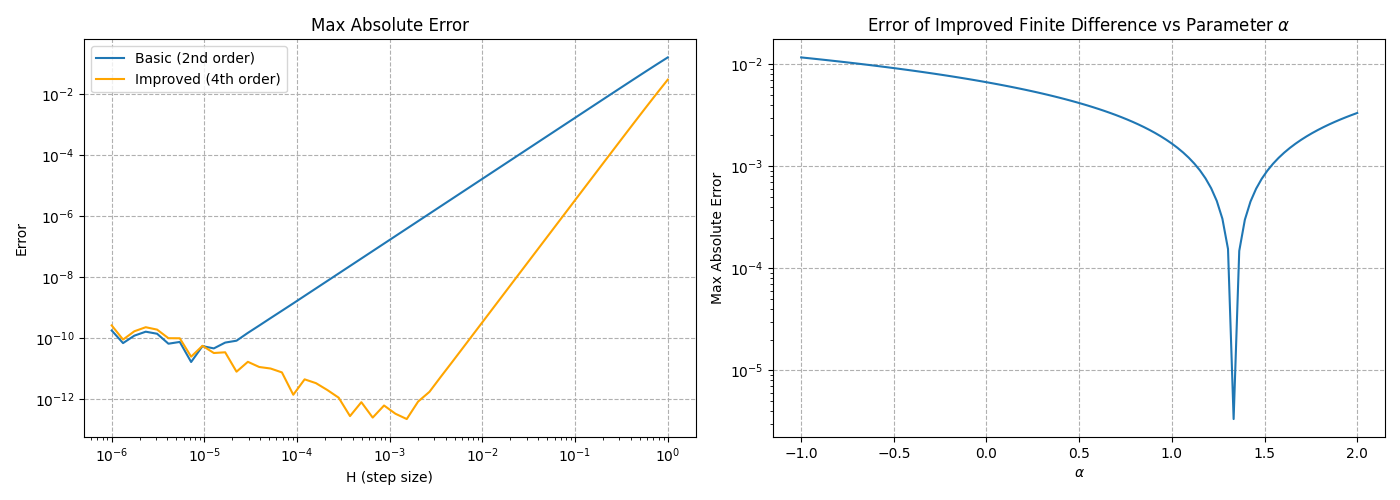
\includegraphics[scale=0.43]{chapters/pm-method/img/finite-difference.png}
    \caption{Left panel: Approximation error for second-order and fourth-order schemes.
        For small values of $H$, round-off errors dominate.
        Right panel: Approximation error vs. $\alpha$ in the improved finite difference scheme ($H = 0.1$).
        Note that the scheme is fourth-order accurate only for $\alpha = 4/3$ (cusp in the graph).}
    \label{fig:finite-diff-accuracy}
\end{figure}

We can alternatively define the finite differences in terms of the delta function to get rid of the dependence on the differenced function. (Technically, the resulting quantities are functions rather than operators.)
Consider, for example, the two-point finite difference in \autoref{eq:two-point-central-diff-def-1} and notice that
\begin{equation*}
    D_j(\phi)(\mathbf{x}) = \frac{\phi(\mathbf{x} + H \mathbf{e}_j)-\phi (\mathbf{x} - H \mathbf{e}_j)}{2H} = \int d\mathbf{x}' \left[ \frac{\delta(\mathbf{x} + H\mathbf{e}_j - \mathbf{x}') - \delta(\mathbf{x} - H\mathbf{e}_j - \mathbf{x}')}{2H} \right]\phi(\mathbf{x}').
\end{equation*}
Thus, we see that
\begin{equation}\label{eq:two-point-central-diff}
    D_j(\mathbf{x}) = \frac{\delta(\mathbf{x} + H\mathbf{e}_j) - \delta(\mathbf{x} - H\mathbf{e}_j)}{2H}
\end{equation}
and
\begin{equation}\label{eq:four-point-central-diff}
    D_j(\mathbf{x}) = \frac{\delta(\mathbf{x} + H\mathbf{e}_j) - \delta(\mathbf{x} - H\mathbf{e}_j)}{2H} + (1-\alpha)\frac{\delta(\mathbf{x} + 2H\mathbf{e}_j) - \delta(\mathbf{x} - 2H\mathbf{e}_j)}{4H}
\end{equation}
are the kernels of the two-point and four-point finite difference operators, respectively.
In symbols,
\begin{equation*}
    \mathbf{D}(\phi)(\mathbf{x}) = \int d\mathbf{x}' \mathbf{D}(\mathbf{x} - \mathbf{x}')\phi(\mathbf{x}').
\end{equation*}

If $\phi$ denotes the gravitational potential, then the field $\mathbf{g}$ is approximated at mesh point $\mathbf{x}_\mathbf{p}$ as
\begin{equation*}
    \mathbf{g}(\mathbf{x}_\mathbf{p}) = -\mathbf{D}(\phi)(\mathbf{x}_\mathbf{p}),
\end{equation*}
which is the discrete version of the relation $\mathbf{g} = -\nabla \phi$.
